\documentclass[11pt,a4paper]{article}
\usepackage[margin=1in]{geometry}
\usepackage[T1]{fontenc}
\usepackage[utf8]{inputenc}
\usepackage{lmodern,microtype}
\usepackage{amsmath,amssymb,amsthm,mathtools}
\usepackage{graphicx,booktabs,tabularx,array,longtable}
\usepackage[authoryear,round]{natbib}
\usepackage{xurl}
\usepackage[hidelinks]{hyperref}
\usepackage[nameinlink,noabbrev]{cleveref}
\usepackage{enumitem}
\graphicspath{{figures/}}
\setlength{\emergencystretch}{2em}
\setlength{\tabcolsep}{5pt}
\renewcommand{\arraystretch}{1.14}
\newcolumntype{Y}{>{\raggedright\arraybackslash}X}
\newtheorem{proposition}{Proposition}
\newtheorem{theorem}[proposition]{Theorem}
\newtheorem{corollary}[proposition]{Corollary}
\newtheorem{lemma}[proposition]{Lemma}
\theoremstyle{definition}
\newtheorem{definition}[proposition]{Definition}
\newtheorem{remark}[proposition]{Remark}
\crefname{remark}{remark}{remarks}
\Crefname{remark}{Remark}{Remarks}
\newcommand{\CITH}{\textsc{CITH}}
\newcommand{\dd}{\,\mathrm{d}}
\newcommand{\ls}{\ell_s}
\newcommand{\Btip}{B_{\rm tip}}
\newcommand{\Blat}{B_{\rm lat}}
\newcommand{\Lmin}{\Lambda_{\min}}
\newcommand{\acrit}{a_{\rm crit}^{\ell}}
\newcommand{\vf}[1]{{\footnotesize\texttt{#1}}}

\title{Fast Minds, Slow Light\\[3pt]
\large Causal Limits on the Growth of Computational Civilizations}
\author{Hyeonjun Joo\\[3pt]\normalsize Independent Researcher, Republic of Korea\\
\normalsize\href{mailto:jonejoo0805@gmail.com}{jonejoo0805@gmail.com}}
\date{14 October 2026 \textemdash{} draft follow-up to \CITH{} v8, for author review}
\hypersetup{pdftitle={Fast Minds, Slow Light: Causal Limits on the Growth of Computational Civilizations},pdfauthor={Hyeonjun Joo}}
\begin{document}\maketitle
\begin{abstract}
The computational inward transition hypothesis (\CITH) treats the delay of
remote returns as a parameter. The speed of light makes that delay geometric
and constrains growth in two further ways. We derive the consequences within
the resource-allocation model of \CITH. First, causality bounds acquired
resources by the content of the light cone: with bounded resource density the
budget grows at most polynomially, any exponential acquisition phase has a
computable maximum duration, and in flat $\Lambda$CDM nothing emitted from now
on can influence matter beyond a comoving radius of 16.7 billion light-years.
A causal cap on the acquisition process of \CITH{} weakly enlarges its inward
basin but cannot undo a crossing of the tipping budget. Second, for a subjective
clock $\omega$ and discount rate $\delta$, the latency length $\ls=c/(\delta\omega)$
converts the robustness ratio $\rho$ into a distance: the corner test for the
nearest opportunity holds exactly when that opportunity lies beyond
$(\ls/\kappa)\ln\rho$. Centrally evaluated frontier expansion therefore stops
at a finite radius, asymptotically $(k/\kappa)\ls\ln\ls$ for resource content
growing as $r^k$, and geographical backups lag by $\omega r/c$ in subjective
time. Third, integration within a subjective round trip $\tau$ confines
computation to a diameter $c\tau/(2\omega)$, so integrated power has a ceiling
falling as $\omega^{-2}$. Combining these channels yields a unique
latency-containment budget, from which $c$ cancels at the fastest
integration-compatible clock. None of these limits binds autonomous
descendants, whose lineages grow as percolation clusters. The speed of light
thus supplies physical reasons for the bounded budgets on which inward
scenarios rely, but not, by itself, an explanation of silence.
\end{abstract}
\noindent\textbf{Keywords:} Fermi paradox; speed of light; latency;
computational civilizations; resource acquisition; percolation; technosignatures.

\section{Introduction}
\label{sec:intro}
The computational inward transition hypothesis asks why a civilization able
to expand would stop paying to do so \citep{Joo2026v8}. Its eighth version
(hereafter v8) answers with a resource-allocation theory: a corner criterion,
a tipping budget, an inward basin, a no-replication criterion, and a
population constraint on the expansionist tail. Distance appears in v8 only
through a parameter. A remote project has an objective delay
$T^{\rm lag}$, a civilization has a subjective clock $\omega$, and the
discount exponent is $\delta\int\omega\dd u$ (v8, eq.~(58) and Proposition~24). Its main
illustration of delay is a four-light-year trip at a tenth of the speed of
light.

The speed of light is not one delay among many. It fixes how fast physical
resources can be acquired, the minimum delay of every remote return, and the
largest region that can compute as a unit. Each of these limits interacts with
the clock. For a mind running $\omega$ times faster than physical time, light
covers $c/\omega$ per subjective second: about $300\,{\rm m\,s^{-1}}$ at
$\omega=10^6$. At that clock one astronomical unit is $15.8$ subjective years
away, and the nearest known stellar system, at about $1.30\,{\rm pc}$
\citep{Reyle2021}, is more than four million subjective years away.
\Citet{Sandberg1999} noted that faster processing makes the internal
light delays of large computing objects subjectively longer, and
\citet{Hanson2016Em} discussed how communication delays would limit the
separation of fast emulated minds in dense cities. This paper turns those
observations into allocation results connected to v8.

\subsection{Contributions}
Each contribution below is conditional on stated assumptions and is proved in
\cref{app:proofs}; numerical checks are listed in \cref{app:numerical}.
\begin{enumerate}[leftmargin=*,itemsep=2pt]
\item \emph{Acquisition} (\cref{sec:acquisition}). Causality bounds acquired
resources by the content of the light cone (\cref{lem:envelope}). With bounded
density the budget is at most polynomial in time, and an exponential phase has
an explicit maximum duration (\cref{cor:exp-phase}). A causal cap on v8's
acquisition process weakly enlarges the inward basin but leaves lock-in
intact (\cref{prop:capped-basin}). In flat $\Lambda$CDM the affectable budget
is finite (\cref{lem:cosmic}).
\item \emph{Latency} (\cref{sec:latency}). Corner tests in replication directions
alone certify no replication (\cref{lem:rep-certificate}). The latency length
turns v8's robustness ratio into a minimum distance to the nearest opportunity
(\cref{prop:latency-radius}). Centrally evaluated frontier expansion stops at
a finite radius scaling as $\ls\ln\ls$ (\cref{prop:frontier}).
Geographical backups are stale by $\omega r/c$ in subjective time (\cref{cor:stale}).
\item \emph{Integration} (\cref{sec:integration}). A computation that must
complete subjective round trips within $\tau$ has a power ceiling falling as
$\omega^{-2}$ (\cref{prop:coherence}). We resolve the coupling of computational
efficiency and clock speed that v8 left as future work (\cref{prop:clock}), and
obtain a latency-containment budget from which $c$ cancels (\cref{thm:containment}).
\item \emph{Decentralization} (\cref{sec:decentral}). Autonomous colonies face
nearest-neighbour delays, not the distance to their origin. Their lineages are
percolation clusters, so restraint must be inherited colony by colony
(\cref{prop:lineage}). Near-light fronts also hide themselves until they
arrive (\cref{rem:visibility}).
\end{enumerate}

\subsection{Relation to prior work}
Physical limits on computation are established subjects. \Citet{Lloyd2000}
bounded the operation rate and memory of a computer by its energy and degrees
of freedom, using the bound of \citet{MargolusLevitin1998}; \citet{Sandberg1999}
reviewed density, speed, dissipation and communication limits on very large
computing objects; and \citet{Bradbury1999} described stellar-scale nested
computers. Cosmological acceleration limits what any civilization can reach or
compute \citep{KraussStarkman2000,ArmstrongSandberg2013,Ord2021}. Expansion
fronts and their visibility have been modelled as bubbles in an expanding
universe \citep{Olson2015,Hanson2021Grabby}; settlement fronts and their
saturation by \citet{NewmanSagan1981} and \citet{CarrollNellenback2019}; and
colonization as percolation by \citet{Landis1998}. Slowing computation as the
universe cools was proposed by \citet{Dyson1979} and, as deliberate waiting, by
\citet{Sandberg2017}. Movement toward dense internal scales was described by
\citet{Smart2012}. The present paper claims no priority for these qualitative
ideas. Its contribution is the set of inequalities that connect them to the
corner, basin, no-replication and population results of v8.

\subsection{Scope}
All results are conditional. We do not estimate subjective clocks, discount
rates, integration tolerances or heat-flux limits for any civilization, and
the examples use scenario values labelled as such. Space is static and
Euclidean except in \cref{sec:cosmic}. Clocks are constant unless stated. For
a non-decreasing clock, v8's integral exponent is at least the value computed
with the clock at the decision time, so every sufficient condition below
remains sufficient.

\section{Causal geometry and subjective scales}
\label{sec:geometry}
\subsection{Inherited objects}
We use v8's notation without change. A civilization allocates a budget $B$
between local investment, with production $a\ell(z)$, and external directions
$j$ with prices $p_j$, initial computational returns $r_j$ and residual slopes
$S_j$. Value is $F_\eta$ with curvature $\eta$; $d_0=1+C_0$,
$\Omega=a\ell(B)$ and $\Gamma=\ell(B)/\ell'(B)$. The all-inward corner is
optimal under concavity exactly when $p_j\geq P_j$ in every direction, where
\begin{equation}
 P_j=\frac{r_j+S_j(d_0+\Omega)^\eta}{a\ell'(B)}
 \label{eq:required-price}
\end{equation}
is the \emph{required price} of v8, Proposition~3. For $\eta=1$ and
$\ell(z)=\ln(1+z)$, $P_j=H_j+A_j/a$ with $H_j=(1+B)\ln(1+B)S_j$ and
$A_j=(1+B)(r_j+d_0S_j)$, and v8's robustness ratio is $\rho=\max_jP_j/p_j$.
The tipping budget $\Btip$ solves $\Gamma(\Btip)=\min_{S_j>0}p_j/S_j$
(v8, Proposition~11).

\subsection{Three lengths}
A project in direction $j$ at distance $r$ has an objective delay
\begin{equation}
 T_j(r)\geq T_j^0+\kappa_j\frac rc,
 \label{eq:delay}
\end{equation}
where $T_j^0\geq0$ collects construction and deployment time. An effect that
must travel out at speed $v\leq c$ has $\kappa_j\geq c/v\geq1$. A payoff that
must also be reported home has $\kappa_j\geq c/v+1\geq2$. For a constant clock
the discount exponent of v8 is $D_j(r)=\delta\omega T_j(r)$.

\begin{definition}[Subjective scales]
\label{def:scales}
For a constant clock $\omega>0$, a subjective discount rate $\delta>0$ and a
subjective integration tolerance $\tau>0$, define the \emph{subjective light
speed} $c/\omega$, the \emph{latency length} and the \emph{coherence diameter}
\begin{equation}
 \ls=\frac{c}{\delta\omega},\qquad
 \Lambda=\frac{c\tau}{2\omega}.
 \label{eq:lengths}
\end{equation}
The latency length is the distance over which a one-way light delay adds one
unit to the discount exponent. The coherence diameter is the largest
separation across which a signal round trip fits within $\tau$ subjective time.
\end{definition}

\begin{lemma}[Scale identity]
\label{lem:scale-identity}
The ratio $\ls/\Lambda=2/(\delta\tau)$ depends only on subjective quantities.
For a computation of diameter $\Lambda$, a round trip $(\kappa=2,T^0=0)$ to
distance $r$ has discount exponent
\begin{equation}
 D=\delta\tau\,\frac r\Lambda .
 \label{eq:scale-identity}
\end{equation}
\end{lemma}
\noindent The proof is division of the two expressions in \cref{eq:lengths}.
The identity explains why the speed of light will cancel from the containment
result of \cref{sec:integration}. Both the size of an integrated computation
and the distance at which it discounts remote returns are proportional to
$c/\omega$.

\Cref{tab:scales} lists the three lengths at three clocks. At $\omega=10^6$, a
subjective day of round-trip tolerance spans about one Earth diameter, and a
subjective year spans $0.032$ astronomical units. \Cref{fig:scales}(a) plots
$\Lambda$ against $\omega$. A kilo-speed clock with a tolerance of $0.1\,$s,
a reaction time, gives $15\,$km. This is the scale of city-size separation
discussed by \citet{Hanson2016Em}.

\begin{table}[tbp]
\centering\small
\caption{Subjective scales for three clocks. One-way light times are in
subjective units. Distances use the IAU astronomical unit and parsec and the
JPL mean Earth radius \citep{JPLPhysical}; $1.30\,$pc is the distance of the
nearest known stellar system \citep{Reyle2021}. Clock speeds and tolerances are
scenarios.}
\label{tab:scales}
\begin{tabular}{@{}lrrr@{}}\toprule
 & $\omega=1$ & $\omega=10^3$ & $\omega=10^6$\\\midrule
Subjective light speed $c/\omega$ (m\,s$^{-1}$) & $2.998\times10^8$ & $2.998\times10^5$ & $299.8$\\
Earth diameter, one way & $0.0425$ s & $42.5$ s & $11.8$ h\\
1 au, one way & $8.32$ min & $5.78$ d & $15.8$ yr\\
1.30 pc, one way & $4.24$ yr & $4{,}240$ yr & $4.24\times10^6$ yr\\\midrule
$\Lambda$ at $\tau=0.1$ s & $1.50\times10^7$ m & $15.0$ km & $15.0$ m\\
$\Lambda$ at $\tau=1$ day & $86.6$ au & $0.0866$ au & $1.30\times10^7$ m\\
$\Lambda$ at $\tau=1$ yr & $0.153$ pc & $31.6$ au & $0.0316$ au\\\bottomrule
\end{tabular}
\end{table}

\begin{figure}[tbp]
\centering
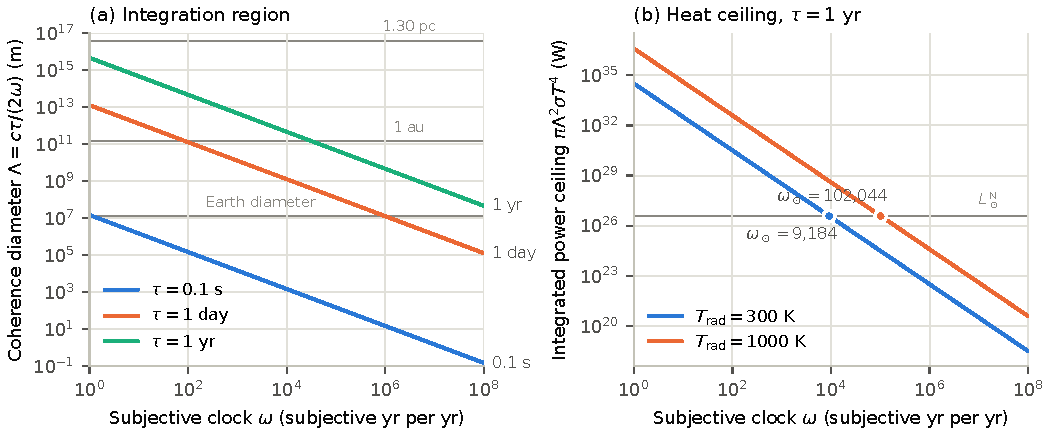
\includegraphics[width=\textwidth]{ls_fig1_scales.pdf}
\caption{(a) Coherence diameter $\Lambda=c\tau/(2\omega)$ for three
subjective tolerances, with reference lengths. (b) The integrated power ceiling
$\pi\Lambda^2\sigma T_{\rm rad}^4$ of \cref{prop:coherence} for $\tau=1$ yr and
two radiator temperatures. Dots mark the clock $\omega_\odot$ above which the
nominal solar luminosity can no longer be dissipated by one integrated
computation. All tolerances, temperatures and clocks are scenarios.}
\label{fig:scales}
\end{figure}

\section{Acquisition: the light-cone budget}
\label{sec:acquisition}
\subsection{The causal envelope}
Place the origin at the centre of a home ball of radius $r_h$. Let $M(r)$ be
the resource content, in v8's budget units, of sites within distance $r$ of the
origin but outside the home ball. Thus $M$ is non-decreasing and vanishes on
$[0,r_h]$. A uniform density $n$ of sites with mean content $\bar b$ gives
$M(r)\approx(4\pi/3)n\bar b\,r^3$. Roughly 340 stellar and substellar systems
lie within $10\,$pc of the Sun \citep{Reyle2021}, a mean system density of
about $0.08\,{\rm pc}^{-3}$. In a disc much wider than it is thick the growth
is quadratic, and beyond a galaxy $M$ has long plateaus.

\begin{lemma}[Causal acquisition envelope]
\label{lem:envelope}
Let an acquisition process be initiated in the home ball at objective time
zero, with no influence propagating faster than $c$. By time $t\geq0$, the
resources at sites it has influenced are at most $M(r_h+ct)$, and the
resources it has delivered back into the home ball are at most
$M(r_h+ct/2)$. If $M(r)\leq Kr^k$ for $r\geq r_h$, then a budget $B(t)$ built
from the home content $B_{\rm home}$ and influenced sites satisfies
\begin{equation}
 B(t)\leq B_{\rm home}+K(r_h+ct)^k,\qquad
 \limsup_{t\to\infty}\frac{\ln B(t)}{t}\leq0.
 \label{eq:envelope}
\end{equation}
\end{lemma}
\noindent Influence must lie in the causal future of the home ball, and a
delivery requires a round trip. The proof is in \cref{app:envelope-proof}.

\begin{corollary}[Finite exponential phase]
\label{cor:exp-phase}
Under the power envelope, if $B(t)\geq B(0)\exp(gt)$ on $[0,T]$ with $g>0$ and
$B(0)>0$, then
\begin{equation}
 T\leq\max\left\{\frac{r_h}{c},\
 \frac{(B_{\rm home}/K)^{1/k}}{2c},\
 2c\left(\frac{2K}{B(0)}\right)^{1/k}\left(\frac{2k}{eg}\right)^2\right\}.
 \label{eq:exp-phase}
\end{equation}
\end{corollary}
\noindent The bound uses $e^y\geq(ey/m)^m$ with $m=2k$; see
\cref{app:envelope-proof}. It applies directly to v8's inward-basin model. In
v8, Proposition~14, a path that reaches the tipping budget satisfies
$B_{t+1}-\Btip>(1+g_X/p)(B_t-\Btip)$ (v8, eq.~(43)), so its excess grows at least
geometrically. With any physical period length and any polynomial envelope,
that runaway is causally consistent only for finitely many periods. The model
needs a cap.

\subsection{A causal cap on the inward basin}
Retain the setting of v8, Proposition~14: one replicating channel,
$p,S>0$, $r\geq0$, $d_0\geq1$, $X_0=0$, a mobilized local budget
$0<\bar B<\Btip$, productivity $a_t=a_0\exp(g_at)$, and the myopic static policy
$x_t=x^*(B_t,a_t)$ of v8, eq.~(42). Replace the acquisition rule by
\begin{equation}
 B_t=\bar B+\min\{g_XX_t,E_t\},\qquad X_{t+1}=X_t+x_t,
 \label{eq:capped}
\end{equation}
where $E_t\geq0$ is non-decreasing. For example, $E_t=M(r_h+c\Delta t/2)$ for a
period of length $\Delta$. Investment beyond the cap is banked as stock in
transit and becomes usable as the cap rises.

\begin{proposition}[A causal cap enlarges the inward basin]
\label{prop:capped-basin}
In the capped model:
\begin{enumerate}[label=(\roman*),leftmargin=*,nosep]
\item every budget path lies below the uncapped path from the same $a_0$, is
non-decreasing in $t$, and is pointwise non-increasing in $a_0$;
\item if the uncapped path from $a_0$ is captured, so is the capped path. The
captured initial productivities form an up-set containing $(a_{\rm sep},\infty)$,
so its infimum, the capped separator, satisfies $a_{\rm sep}^{\rm cap}\leq a_{\rm sep}$;
\item no capped path reaches $\Btip$ before $t_E=\min\{t:\bar B+E_t\geq\Btip\}$,
and if $\bar B+\sup_tE_t<\Btip$ every positive $a_0$ is captured;
\item once a capped path reaches $\Btip$, new external investment is positive in
every later period, while $B_t\leq\bar B+E_t$.
\end{enumerate}
\end{proposition}
\noindent The proof inducts on $t$, using v8's monotonicity of $x^*$ in budget and
productivity (\cref{app:capped-proof}). Light speed thus delays lock-in and
caps its growth rate, but cannot reverse a crossing.

\Cref{tab:capped} applies the cap to v8's numerical example. Slower envelopes
lower the separator from $6.632$ to about $4.33$, but not to zero. While the
cap binds, a low-productivity path keeps investing for the residual payoff $Sx$.
The banked stock becomes usable as the light cone grows, and the path then
crosses the tipping budget. Only a bounded envelope, as in (iii), captures
every path.

\begin{table}[tbp]
\centering\small
\caption{v8's example $(p,S,r,d_0)=(1,0.002,0.05,1)$, $g_a=0.05$, $g_X=0.5$,
$\bar B=0.6\Btip$, with the cubic cap $E_t=e_3t^3$. Here $t_E$ is the first
period at which the cap could admit $\Btip$. The uncapped separator is
$6.632159$. Separators are bisected on certified capture or crossing.}
\label{tab:capped}
\begin{tabular}{@{}rrr@{}}\toprule
$e_3$ & $t_E$ & $a_{\rm sep}^{\rm cap}$\\\midrule
$1$ & $3.49$ & $6.612150$\\
$10^{-1}$ & $7.51$ & $6.454066$\\
$10^{-2}$ & $16.19$ & $5.882275$\\
$10^{-3}$ & $34.87$ & $4.950497$\\
$10^{-4}$ & $75.13$ & $4.404970$\\
$10^{-5}$ & $161.85$ & $4.334291$\\\bottomrule
\end{tabular}
\end{table}

\subsection{A cosmological ceiling}
\label{sec:cosmic}
\begin{lemma}[Finite affectable budget]
\label{lem:cosmic}
In a flat Friedmann--Lema\^{\i}tre--Robertson--Walker universe with
$H(a)=H_0E(a)$, $E(a)=[\Omega_ra^{-4}+\Omega_ma^{-3}+\Omega_\Lambda]^{1/2}$ and
$\Omega_\Lambda>0$, a signal emitted at scale factor $a_e$ reaches comoving distance at most
\begin{equation}
 \chi_{\rm EH}(a_e)=\frac c{H_0}\int_{a_e}^\infty\frac{\dd a}{a^2E(a)}
 \leq\frac{c}{H_0a_e\sqrt{\Omega_\Lambda}},
 \label{eq:event-horizon}
\end{equation}
and material probes reach strictly less. If usable resources have bounded
comoving density $\bar n$, every budget built from sites influenced after
today is at most $B_{\rm home}+(4\pi/3)\bar n\chi_{\rm EH}(1)^3$.
\end{lemma}
\noindent For the Planck 2018 base-$\Lambda$CDM values $H_0=67.4\,{\rm
km\,s^{-1}\,Mpc^{-1}}$ and $\Omega_m=0.315$ \citep{Planck2020}, flat and without
radiation, $\chi_{\rm EH}(1)=16.68$ billion light-years ($5.11\,$Gpc), against
the bound $17.53$. The particle horizon is $47.0$ billion light-years ($46.1$
with a radiation density of $9.2\times10^{-5}$ of critical). The affectable
comoving volume is therefore $4.5$--$4.8$ per cent of the currently observable
volume. These are kinematic statements, consistent with
\citet{KraussStarkman2000} and \citet{Ord2021}.

The consequence for \CITH{} is logical rather than practical. v8's
unbounded-budget theorems (Proposition~8 and Corollaries~9 and~19) describe
intermediate regimes. The final classification compares a bounded budget
with the tipping budget (v8, Proposition~11) or with its ceiling version
(Corollary~12). Since $\Gamma(B)\geq B$, the tipping budget is at most
$\min_jp_j/S_j$. A cosmic budget therefore helps all-inward allocation only if
residual slopes are smaller than $p_j/B_{\rm reach}$, which is extraordinarily
small.

\section{Latency: remote returns on a subjective clock}
\label{sec:latency}
\subsection{Replication tests certify no replication}
The latency results concern replication. Observation and dormant backups may
remain active at short range, so we first separate the two.

\begin{lemma}[Corner tests certify no replication]
\label{lem:rep-certificate}
Take v8's model with observation and backups (v8, eq.~(51) and Proposition~20):
concave $\ell$ and residual functions, and strictly increasing concave $F$. Suppose a
no-replication face optimizer exists with finite derivatives. If each
replication direction $j\in\{n,h\}$ passes its all-inward corner test,
\begin{equation}
 F'(C_L)r_j+S_j\leq p_jF'(C_L)a\ell'(B),\qquad C_L=C_0+a\ell(B),
 \label{eq:rep-corner}
\end{equation}
then a no-replication optimizer is globally optimal. Strict inequalities exclude
replication from every full optimizer. This holds whatever the observation and backup
prices, and whether or not those channels pass their own corner tests.
\end{lemma}
\noindent The face multiplier satisfies $\lambda\geq F'(C^*)a\ell'(z^*)\geq
F'(C^*)a\ell'(B)$, while $F'(C^*)\geq F'(C_L)$ and $R'(b^*)\leq R'(0)$,
$I'(w^*)\leq I'(0)$. Together these bounds show that \cref{eq:rep-corner} implies v8's
no-replication inequalities (\cref{app:rep-proof}). The converse is false. In 1,200
random instances in the validator, 79 have no replication despite failing a
replication corner test. On v8's frozen 1,024-row design, the 333 rows
certified by \cref{eq:rep-corner} lie within v8's 421 no-replication rows, with
no exception.

\subsection{The latency radius}
Extend v8's static model to finitely many distance classes. Direction $j$ is
available at distances $r$ in a finite set $\mathcal R_j$, at price $p_j(r)$.
At the all-inward corner, the right derivative of utility in that direction is
$e^{-D_j(r)}[F'(C_L)r_j+S_j]$: v8's undiscounted return, attenuated by the
discount exponent of the delay \cref{eq:delay}. Utility is concave.

\begin{proposition}[Latency radius]
\label{prop:latency-radius}
The corner is optimal exactly when $p_j(r)\geq e^{-D_j(r)}P_j$ for every $j$
and every $r\in\mathcal R_j$, with $P_j$ from \cref{eq:required-price}. If each
$p_j$ is non-decreasing in distance, only the nearest distance
$r_j^{\min}=\min\mathcal R_j$ matters. For a constant clock, the corner holds
exactly when, in every direction with $\rho_j=P_j/p_j(r_j^{\min})>1$,
\begin{equation}
 r_j^{\min}\geq r_{{\rm lat},j}=\frac{\ls}{\kappa_j}
 \left[\ln\rho_j-\delta\omega T_j^0\right].
 \label{eq:latency-radius}
\end{equation}
By \cref{lem:rep-certificate}, the same inequality imposed on replication
directions alone certifies no replication.
\end{proposition}
\noindent This is v8, Proposition~3, applied to the enlarged set of directions
(\cref{app:latency-proof}). The geometric content is the conversion: v8's
robustness ratio becomes a distance, measured in latency lengths. Raising
productivity shortens the latency radius only logarithmically.

\Cref{fig:design} applies a common delay exponent $D$ to every external
direction of v8's frozen design. This would be the case if all opportunities
lay at the nearest system. The all-inward count rises from $219$ at $D=0$ to
all $1{,}024$ rows at $D=8.539$, the largest $\ln\rho$ in the design. Rows
certified by \cref{lem:rep-certificate} rise from $333$ and reach $1{,}024$ at
$D=7.950$. The exact restricted-face count rises from v8's $421$ and reaches
$1{,}024$ by $D=8$. For a constant clock, $\kappa=2$ and a nearest system at
$1.30\,$pc, every row is all-inward once $\ls\leq0.3045\,$pc, that is, once
$\delta\omega\geq1.007$ per objective year. At $\omega=10^6$ this is
$\delta\approx1.0\times10^{-6}$ per subjective year, the order of the
thresholds in v8's Table~1. As in v8, these counts check an implementation on
a frozen synthetic design. They are not prevalence estimates.

\begin{figure}[tbp]
\centering
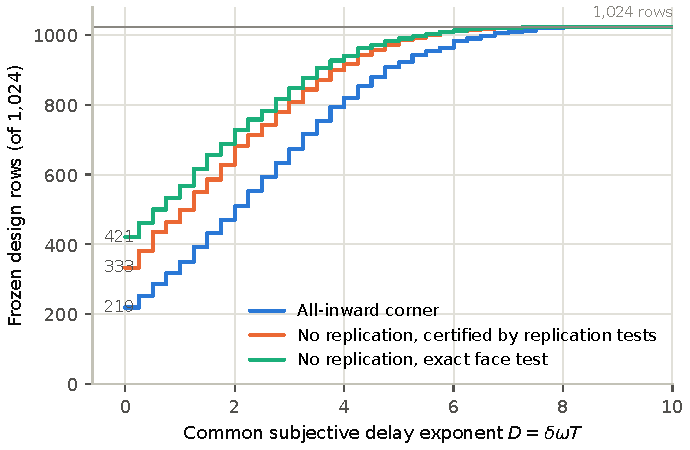
\includegraphics[width=.72\textwidth]{ls_fig2_design.pdf}
\caption{Rows of v8's frozen design that pass, under a common subjective delay
exponent $D$ applied to every external return and residual slope. The three
tests are the all-inward corner, the replication-only certificate of
\cref{lem:rep-certificate}, and the exact no-replication test on the
observation face. For a constant clock, $D=\kappa r_1/\ls$. Values at $D=0$
reproduce v8 exactly.}
\label{fig:design}
\end{figure}

\subsection{Central frontier expansion stops}
Let a civilization hold every site within a frontier radius $R$ and evaluate
all projects centrally. Its budget $B(R)$ may grow with $R$ through imported
resources. Its replication opportunities lie at distances at least $R$. A
replication direction at distance $r$ enters \cref{lem:rep-certificate} with
computational return $e^{-D_j(r)}r_j$ and residual slope $e^{-D_j(r)}S_j$, and
its marginal value at any face allocation is bounded by these discounted values.
Observation and backups at held sites are left unrestricted.

\begin{proposition}[Self-limiting central expansion]
\label{prop:frontier}
Assume $0\leq\eta\leq1$; concave $\ell$ with $\Gamma(B)\leq K_\Gamma(1+B)^m$
for $B\geq B_0:=B(0)$; productivity $a\geq a_{\min}>0$; prices at least
$p_{\min}>0$; undiscounted coefficients $r_j\leq\bar r$ and $S_j\leq\bar S$,
possibly varying with $R$; budgets $B_0\leq B(R)\leq B_0+K(1+R)^k$; and discount
exponents $D_j(r)\geq\kappa r/\ls$ with $\kappa>0$. Put
$K_1=(\bar r+d_0\bar S)/(a_{\min}\ell(B_0))+\bar S$ and
\begin{equation}
 \bar R=\sup\Big\{R\geq0:\ \frac{\kappa R}{\ls}\leq
 \ln\frac{K_1K_\Gamma[1+B_0+K(1+R)^k]^m}{p_{\min}}\Big\}.
 \label{eq:Rbar}
\end{equation}
\begin{enumerate}[label=(\roman*),leftmargin=*,nosep]
\item $\bar R<\infty$. For every $R>\bar R$ every replication direction passes
strictly, so no full optimizer at frontier $R$ replicates.
\item $\limsup_{\ls\to\infty}\bar R/(\ls\ln\ls)\leq km/\kappa$. For logarithmic
production any $m>1$ is admissible, so the bound is $k/\kappa$.
\item In v8's one-channel benchmark, with logarithmic production and value,
constant $a,p,r,S$ and $r+S>0$, $B(R)=B_0+KR^k$ and $D(R)=\kappa R/\ls$, the
largest radius at which expansion is optimal satisfies
\begin{equation}
 R_{\rm stop}=\frac k\kappa\,\ls\ln\ls\left[1+O\!\left(\frac{\ln\ln\ls}{\ln\ls}\right)\right].
 \label{eq:Rstop}
\end{equation}
\end{enumerate}
\end{proposition}
\noindent Delay grows linearly in the frontier radius, while the obstruction of
v8 grows like $B\ln B$, only polynomially in $R$. Exponential discounting
therefore wins (\cref{app:frontier-proof}). In physical units, with lengths
measured in a fixed unit $\ell_0$ implicit in $K$,
$R_{\rm stop}\approx(kc/\kappa\delta\omega)\ln[c/(\delta\omega\ell_0)]$. The
size of a centrally governed civilization scales with the speed of light, up to
a logarithm. Letting $\ls\to\infty$, with instantaneous returns, recovers the
growth obstruction of v8, Proposition~8.

\Cref{fig:frontier} uses scenario values: the v8 coefficients with $a=5$,
$B_0=0.6\Btip$, $K=4.1$ budget units per pc$^3$, $k=3$, $\kappa=2$ and
$r_1=1.30\,$pc. The radius reached from the home matches $R_{\rm stop}$ once
expansion starts. It starts only for $\ls>7.754\,$pc. For
$4.24\lesssim\ls<7.754\,$pc, expansion would pay at radii of 10--30 pc, but the
first step to $1.30\,$pc does not. Latency can thus stop growth at the first
step even when a larger civilization would keep expanding. The ratio
$R_{\rm stop}/(\ls\ln\ls)$ converges slowly, from $2.12$ at $\ls=10$ to $1.69$
at $\ls=10^{14}$ in the same units. The scaled deviation in \cref{eq:Rstop}
stays between $1.70$ and $1.72$, as the proof predicts.

\begin{figure}[tbp]
\centering
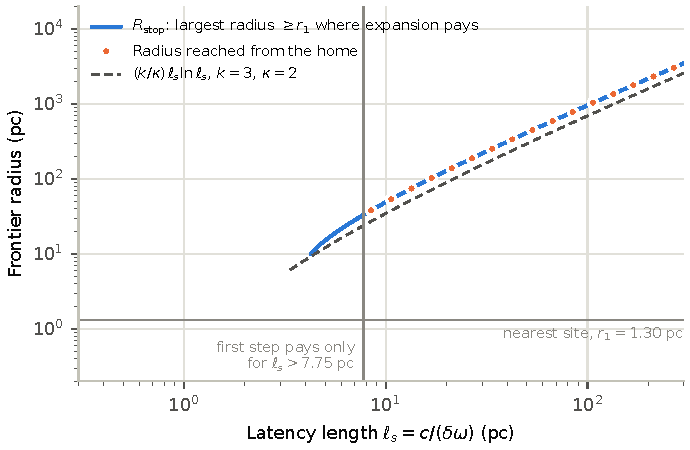
\includegraphics[width=.72\textwidth]{ls_fig3_frontier.pdf}
\caption{Central frontier expansion in the one-channel benchmark. The line is
the largest radius beyond the nearest site at which expansion is optimal. Dots
mark the radius actually reached from the home. The dashed curve is the
leading asymptote of \cref{eq:Rstop}. All parameters are scenarios.}
\label{fig:frontier}
\end{figure}

\subsection{Stale backups}
Light speed also limits geographical insurance. A backup at distance $r$ can be
updated only by signals. At a catastrophe it therefore restores the home state
as of at least $r/c$ earlier, which is $\omega r/c$ in subjective time.

\begin{corollary}[Stale geographical backups]
\label{cor:stale}
In v8's endogenous-risk model (Proposition~23), let the restored value be
$\psi F_\eta(C)$ with $\psi=\Psi(\omega r/c)\in[0,1]$, where $\Psi$ is non-increasing
and $\Psi(0)=1$. Then the necessary condition for no backup is v8, eq.~(55),
with $\varphi'(0)$ replaced by $\psi\varphi'(0)$:
\begin{equation}
 p\geq\frac{\Gamma r}{\Omega}
 +\frac{\vartheta}{1-\vartheta}\psi\varphi'(0)\Gamma\Omega^{-\gamma}K_\eta(\Omega).
 \label{eq:stale}
\end{equation}
The limiting hazard ceiling becomes
$\vartheta\leq p(1-\eta)/[p(1-\eta)+\psi\varphi'(0)\Gamma]$. If valued internal
state grows at subjective rate $g$, then $\Psi(u)=e^{-gu}$, and staleness acts as
subjective discounting at rate $g$ over the one-way light time, even when $\delta=0$.
\end{corollary}
\noindent At $\omega=10^6$, a backup at $1.30\,$pc lags by $4.24$ million
subjective years. Interstellar insurance of a fast civilization therefore
insures its remote past. A mirror that runs forward independently is not
stale, but it diverges: it is a separate lineage, treated in
\cref{sec:decentral}.

\section{Integration: how large can a fast mind be?}
\label{sec:integration}
\subsection{A coherence ceiling}
\begin{definition}[Integration]
\label{def:integration}
A computation occupying a bounded set $\Sigma\subset\mathbb R^3$ is
\emph{$\tau$-integrated} at clock $\omega$ if every pair of its points can
complete a signal round trip within subjective time $\tau$:
$2|x-y|\omega/c\leq\tau$. Then ${\rm diam}\,\Sigma\leq\Lambda$.
\end{definition}
Signals in matter are slower than $c$, so the definition is optimistic. The
tolerance $\tau$ is a property of the computation: a fraction of a second for
one mind, perhaps days or years for a coordinated society.

\begin{lemma}[Hull geometry]
\label{lem:hull}
If ${\rm diam}\,\Sigma\leq\Lambda$, the convex hull of $\Sigma$ has surface
area at most $\pi\Lambda^2$, with equality for a ball of diameter $\Lambda$.
\end{lemma}
\noindent By Cauchy's formula, the surface area of a convex body in
$\mathbb R^3$ is four times its mean projected area \citep{Schneider2014}. Each
projection has diameter at most $\Lambda$, hence area at most $\pi\Lambda^2/4$
by the planar isodiametric inequality \citep{Bieberbach1915}.

\begin{proposition}[Coherence ceiling on integrated power]
\label{prop:coherence}
Suppose a $\tau$-integrated computation at clock $\omega$ rejects its
dissipated power, in steady state, only across the boundary of its convex
hull, with outward heat-flux density at most $q_{\max}$. Then
\begin{equation}
 P\leq\pi q_{\max}\Lambda^2=\frac{\pi q_{\max}c^2\tau^2}{4\omega^2}.
 \label{eq:coherence}
\end{equation}
For thermal radiation from surfaces no hotter than $T_{\rm rad}$ into a
negligible background, $q_{\max}=\sigma T_{\rm rad}^4$. If every logically
irreversible bit erasure ultimately rejects at least $k_BT_{\rm rad}\ln2$ at the
rejection temperature, then the erasure rate is at most
$\pi\sigma T_{\rm rad}^3c^2\tau^2/(4k_B\omega^2\ln2)$.
\end{proposition}
\noindent The proof combines energy balance, \cref{lem:hull}, the blackbody
bound on thermal emission, the Landauer cost \citep{Landauer1961} and the
Carnot cost of pumping heat to the radiator (\cref{app:coherence-proof}).
Reversible logic avoids the erasure term \citep{Bennett1982}, but not the power
bound. A tenfold faster clock lowers the integrated power ceiling a
hundredfold. Power $P$ can be integrated only at clocks
\begin{equation}
 \omega\leq\omega_P=\frac{c\tau}{2\Lmin(P)},\qquad
 \Lmin(P)=\sqrt{\frac{P}{\pi q_{\max}}}.
 \label{eq:omega-P}
\end{equation}
For the nominal solar luminosity \citep{IAU2015} and $\tau=1\,$yr,
$\omega_\odot=9{,}184$ with $T_{\rm rad}=300\,$K ($\Lmin=3.44\,$au), and
$\omega_\odot=102{,}044$ with $1000\,$K ($0.310\,$au)
(\cref{fig:scales}b). Heat carried away by ejected matter is excluded by
assumption. An engineered coolant might reach a larger $q_{\max}$, but the
$\omega^{-2}$ scaling holds for any fixed $q_{\max}$.

\begin{remark}[Surplus power]
\label{rem:surplus}
For \CITH, \cref{prop:coherence} supplies a physical local ceiling for
integrated computation, $\bar B(\omega)=P_{\max}(\omega)\Delta/b_{\rm ref}$
for a planning horizon $\Delta$. This is the bounded-budget regime in which v8
finds a tipping budget. Growing an integrated civilization requires slowing
it down, since $\omega_P\propto P^{-1/2}$. The ceiling cuts both ways. If local
production is capped at $\bar B(\omega)<B$, its left derivative at $B$ vanishes.
v8's necessary corner condition $F'(C_L)r_j+S_j\leq p_j\lambda_L=0$ then fails in
every direction with positive value. Surplus beyond the integrated capacity
has no integrated use. It can be left unharvested, run by separate,
non-integrated minds, or spent externally. In the last case v8's no-replication
comparison of substitute bundles (Corollary~21) decides whether that spending
replicates.
\end{remark}

\subsection{Clock speed against efficiency}
v8 closes with an open trade-off. If energy efficiency is obtained through
slower adiabatic or reversible computation, productivity $a$ and the clock
$\omega$ are coupled, and raising $a$ can weaken the delay mechanism. In
Brownian and adiabatic computing, dissipation per step grows with the speed of
the step \citep{Bennett1982}. We model the coupling as
\begin{equation}
 a(\omega)=\Xi\,\omega^{-\alpha},\qquad 0\leq\alpha\leq1,\quad
 \omega\geq\omega_{\rm lo}>0,
 \label{eq:coupling}
\end{equation}
with $\alpha=1$ for dissipation proportional to speed. For $\eta=1$ and
logarithmic production, the latency-discounted required price of a replication
direction with delay $T$ is, by v8, Corollary~6,
\begin{equation}
 g(\omega)=e^{-\beta\omega}\Big[H+\frac A\Xi\,\omega^\alpha\Big],\qquad
 \beta=\delta T.
 \label{eq:g}
\end{equation}

\begin{proposition}[Clock speed and efficiency]
\label{prop:clock}
On $[\omega_{\rm lo},\infty)$, $g$ is either strictly decreasing or strictly
increasing and then strictly decreasing, and $g(\omega)\to0$.
\begin{enumerate}[label=(\roman*),leftmargin=*,nosep]
\item The corner set $\{\omega\geq\omega_{\rm lo}:g(\omega)\leq p\}$ is
$[\omega_{\rm lo},\omega_-]\cup[\omega_+,\infty)$ with $\omega_+<\infty$. The
first interval may be empty.
\item If $\alpha=0$, the corner set is $[\omega_+,\infty)$.
\item If $\alpha>0$ and $g(\omega_{\rm lo})\leq p<\max g$, the corner holds for
slow and for fast clocks, but fails on the band $(\omega_-,\omega_+)$.
\item As $\omega_{\rm lo}\to0$ with $\alpha>0$, $g(\omega_{\rm lo})\to H$. The slow
branch therefore exists asymptotically exactly when $p>H$, that is, when
$B<\Btip$.
\item For $\alpha=1$ and $\hat\omega=1/\beta-H\Xi/A>0$, the maximum is
$g(\hat\omega)=(A/\Xi\beta)\exp(\beta H\Xi/A-1)$.
\end{enumerate}
\end{proposition}
\noindent Exponential discounting eventually defeats any polynomial loss of
efficiency, so the coupling never removes the fast route to inwardness. The
efficient slow branch, however, only reproduces v8's tipping comparison, and
an intermediate band of clocks is the worst place to be
(\cref{fig:clock}a; \cref{app:clock-proof}). Which clock a civilization chooses
depends on how it values speed. If only computation is valued and hardware is
plentiful, efficiency favours slow clocks
\citep{Dyson1979,Sandberg2017}. That is exactly where latency protection is
weakest.

\subsection{The light-speed containment budget}
\begin{theorem}[Integration-compatible latency containment]
\label{thm:containment}
Let a civilization dissipate its entire budget $B$, energy per horizon
$\Delta$ in units $b_{\rm ref}$, in one $\tau$-integrated computation under the
flux limit of \cref{prop:coherence}. Let productivity $a$ be fixed, and let
every replication direction have its nearest opportunity at $r_1$ with delay
$\kappa r_1/c$. Let $\rho(B)$ be v8's undiscounted robustness ratio over
replication directions, and suppose every clock up to
$\omega_{\max}(B)=c\tau/[2\Lmin(B)]$, with
$\Lmin(B)=[Bb_{\rm ref}/(\pi q_{\max}\Delta)]^{1/2}$, is available.
\begin{enumerate}[label=(\roman*),leftmargin=*,nosep]
\item Some integration-compatible clock makes every replication direction pass
its latency-discounted corner test exactly when
\begin{equation}
 \frac{\kappa\delta\tau}{2}\,\frac{r_1}{\Lmin(B)}\geq\ln\rho(B).
 \label{eq:containment}
\end{equation}
The speed of light does not appear.
\item If $\rho$ is continuous, non-decreasing and unbounded, as in v8's baseline
with a positive residual slope, the budgets satisfying \cref{eq:containment} form
an interval $(0,\Blat]$ with a unique $0<\Blat<\infty$. Moreover
$\Blat\geq B^{(0)}=\sup\{B:\rho(B)\leq1\}$, and $\Blat$ is non-decreasing in
$r_1$, $\kappa$, $\delta\tau$ and $q_{\max}$.
\item With coupled efficiency \cref{eq:coupling}, $\alpha\in(0,1]$, and clocks in
$[\omega_{\rm lo},\omega_{\max}(B)]$ with $\omega_{\rm lo}\leq\omega_{\max}(B)$, a
containing clock exists exactly when
$\min\{g(\omega_{\rm lo}),g(\omega_{\max}(B))\}\leq p$. The speed of light then
re-enters through $\omega_{\max}(B)^\alpha$.
\end{enumerate}
\end{theorem}
\noindent At the fastest admissible clock the exponent is
$\delta\omega_{\max}\kappa r_1/c=(\kappa\delta\tau/2)r_1/\Lmin(B)$. This is
\cref{lem:scale-identity} with $\Lambda=\Lmin$ (\cref{app:containment-proof}).
The speed of light sets the scales: how fast a civilization can think and how
far away its neighbours feel. Whether an integrated civilization can be
contained by latency depends instead on a geometric ratio. That ratio is the
distance to the nearest opportunity divided by the smallest body able to
radiate the civilization's power, multiplied by the subjective constant
$\kappa\delta\tau/2$. A larger $c$ would allow faster clocks and shorten
delays in exactly offsetting proportion. If a technological speed limit below
$\omega_{\max}(B)$ binds instead, it replaces $\omega_{\max}(B)$ in the test,
and $c$ re-enters.

\Cref{tab:containment} and \cref{fig:clock}(b) use the v8 one-channel
coefficients with $a=50$, $r_1=1.30\,$pc and $\kappa=2$. Without latency, the
corner holds up to $B^{(0)}=96.95$ budget units, $0.80$ of a solar luminosity
sustained for a year. The nominal solar luminosity can be latency-contained
once $\delta\tau\geq3.3\times10^{-6}$ with 300\,K radiators, or
$\geq3.0\times10^{-7}$ at 1000\,K. Here $\delta\tau$ is the subjective
discount rate times the subjective tolerance, both in years. Splitting the
budget among $N$ separate computations divides $\Lmin$ by $\sqrt N$ and does
not raise $\rho$. Many small, fast minds are therefore more easily contained
than one large integrated mind. This is the geometric form of the inward
scenario. Each small mind is, however, a separate decision-maker.

\begin{table}[tbp]
\centering\small
\caption{Containment budget $\Blat$ of \cref{thm:containment} for the v8
one-channel coefficients $(p,S,r,d_0,a)=(1,0.002,0.05,1,50)$, $r_1=1.30\,$pc,
$\kappa=2$, $b_{\rm ref}=10^{32}\,$J and a Julian-year horizon, in budget units
and in nominal solar luminosity-years ($120.8$ units). Radiative flux limits are
scenarios.}
\label{tab:containment}
\begin{tabular}{@{}rrrrr@{}}\toprule
 & \multicolumn{2}{c}{$T_{\rm rad}=300$ K} & \multicolumn{2}{c}{$T_{\rm rad}=1000$ K}\\
$\delta\tau$ & $\Blat$ & $L_\odot$-yr & $\Blat$ & $L_\odot$-yr\\\midrule
$10^{-8}$ & $97.02$ & $0.803$ & $97.74$ & $0.809$\\
$10^{-6}$ & $104.1$ & $0.862$ & $177.8$ & $1.47$\\
$10^{-4}$ & $1.003\times10^3$ & $8.30$ & $2.347\times10^4$ & $194$\\
$10^{-2}$ & $7.411\times10^5$ & $6.14\times10^3$ & $4.430\times10^7$ & $3.67\times10^5$\\
$1$ & $2.170\times10^9$ & $1.80\times10^7$ & $1.721\times10^{11}$ & $1.42\times10^9$\\\bottomrule
\end{tabular}
\end{table}

\begin{figure}[tbp]
\centering
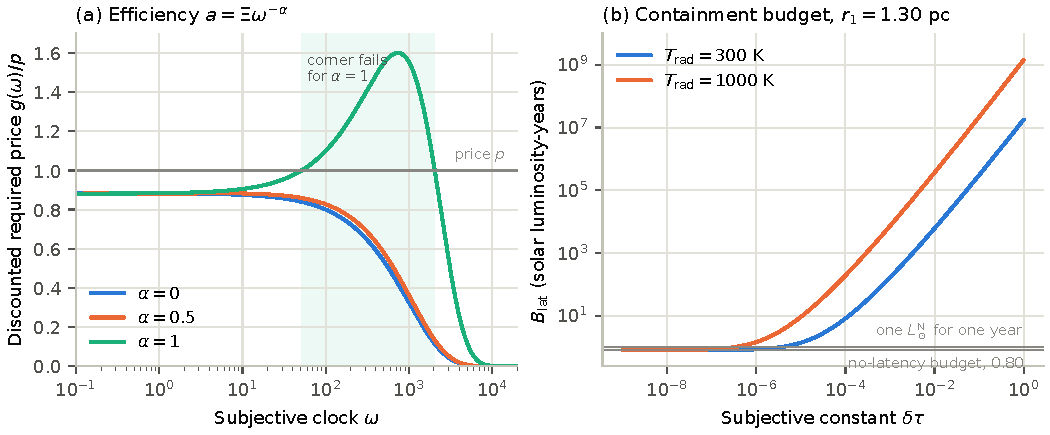
\includegraphics[width=\textwidth]{ls_fig4_clock_containment.pdf}
\caption{(a) Latency-discounted required price, relative to the actual price,
under the efficiency coupling \cref{eq:coupling}, at $B=0.9\Btip$ with
$\beta=10^{-3}$ and $\Xi=1{,}500$. For $\alpha=1$ the corner fails on
$51.5<\omega<2{,}042$ but holds for slower and faster clocks. (b) The
containment budget $\Blat$ of \cref{thm:containment} against the subjective
constant $\delta\tau$. All parameters are scenarios.}
\label{fig:clock}
\end{figure}

\section{Decentralized growth: what light speed cannot contain}
\label{sec:decentral}
\subsection{Colonies evaluate their own frontier}
A colony beyond the coherence diameter cannot be steered from home in real
time. The home's preferences reach it only through what was built in at its
founding, through messages delayed by at least $r/c$, or through physical
enforcement that is itself delayed. A colony that evaluates its own
opportunities applies \cref{prop:latency-radius} with its own nearest-neighbour
distance, not with its distance from the origin. The self-limitation of
\cref{prop:frontier} then has no purchase, and growth becomes a question about
the colony-level decision.

\begin{proposition}[Lineages of autonomous colonies]
\label{prop:lineage}
Let sites be the vertices of an infinite connected graph $G$ of maximum degree
$\Delta\geq2$, with sites one jump apart adjacent. The home is settled and
founds colonies at all its neighbours. Each newly founded colony is
independently an \emph{expander} with probability $\pi$, founding colonies at
all its unsettled neighbours, or founds none.
\begin{enumerate}[label=(\roman*),leftmargin=*,nosep]
\item If $\pi\in\{0,1\}$, as for identical deterministic colonies, the lineage
is either the home and its neighbours or every vertex of $G$. A causal envelope
(\cref{lem:envelope}) bounds the speed of the front. The colony-level test
decides the outcome. The home's stopping radius does not.
\item If $(\Delta-1)\pi<1$, the lineage is finite almost surely, and
\begin{equation}
 \mathbb E[\#\text{settled}]\leq1+\Delta+\frac{\Delta(\Delta-1)\pi}{1-(\Delta-1)\pi},
 \label{eq:lineage-bound}
\end{equation}
with equality on the $\Delta$-regular tree.
\item If $\pi$ exceeds the site-percolation threshold $p_c^{\rm site}(G)$, the
lineage is infinite with positive probability. On the cubic lattice
$p_c^{\rm site}\simeq0.3116$ \citep{DengBlote2005}. On the $\Delta$-regular tree
$p_c^{\rm site}=1/(\Delta-1)$.
\end{enumerate}
\end{proposition}
\noindent Expanders form a branching process dominated by binomial offspring,
and the settled set is an open site-percolation cluster with its boundary
(\cref{app:lineage-proof}; \citealp{Grimmett1999}). In the validator, simulated
mean lineage sizes on regular trees match \cref{eq:lineage-bound}. On the cubic
lattice the means at $\pi=0.10$, $0.15$ and $0.19$ are $11.8$, $17.1$ and
$25.7$, below the tree bounds $13$, $25$ and $121$. Lineages reached distance 30
in $94.5$ per cent of runs at $\pi=0.45$ and in none at $\pi=0.2$.

The implication for \CITH{} is a second uniformity requirement. v8,
Proposition~27, bounds the expansionist fraction among independent origins.
\Cref{prop:lineage} adds a bound inside each lineage that has begun. Long jump
ranges make it stringent. At $0.08$ systems per pc$^3$, a jump range of $5\,$pc
contains about $42$ systems on average. With a maximum degree of that order,
the subcritical condition of (ii) asks that fewer than about one colony in $41$
become an expander. Causal separation
also lets values drift independently in each colony, so restraint that relies
on shared values must be inherited colony by colony. These conditions sit
alongside, not in place of, the population constraint of v8.

\subsection{Near-light fronts hide themselves}
\begin{remark}[Visibility of near-light fronts]
\label{rem:visibility}
In static Euclidean space, let origins form a homogeneous Poisson process in
space-time with intensity $\zeta$, and let each origin launch a spherical front
at speed $v<c$. For an observer at time $t_0$, consider two counts: fronts that
have arrived, and origins visible but not yet arrived. They are independent
Poisson variables with means $(\pi/3)\zeta v^3t_0^4$ and
$(\pi/3)\zeta(c^3-v^3)t_0^4$. Their ratio is $(c/v)^3-1$. Under v8's null-arrival
allowance $\mathcal L_*=-\ln P_*$, the expected number of visible but not yet
arrived expanders is at most $[(c/v)^3-1]\mathcal L_*$. For $P_*=0.05$ this is
$1.1$ at $v=0.9c$ and $0.092$ at $v=0.99c$.
\end{remark}
\noindent The origin event is the first part of a bubble whose light reaches
the observer, which gives the two regions of the past light cone
(\cref{app:visibility-proof}). \Citet{Olson2015} and \citet{Hanson2021Grabby}
develop cosmological versions. Light speed hides fast growth until it arrives.
For near-light fronts, null visibility adds little to null arrival.

\section{Discussion}
\label{sec:discussion}
\Cref{tab:summary} collects the four channels. The speed of light helps an
inward scenario in three ways. It supplies physical reasons for bounded
budgets: the cosmological ceiling, polynomial acquisition, and the coherence
ceiling on integrated computation. It makes latency a consequence of
geometry rather than a free parameter. And it ties fast
clocks to small integrated sizes, so that growth of an integrated
civilization is, in the sense of \citet{Smart2012}, a densification.

It does not fix the preference parameters on which the latency mechanism
rests: the subjective discount rate, the integration tolerance and the clock.
v8 already noted that subjective-time discounting is optional. The
containment criterion \cref{eq:containment} shows that the speed of light
cannot replace such a preference, since it cancels. Light speed also leaves
surplus power without an integrated use (\cref{rem:surplus}), which can favour
external projects. Above all it cannot stop autonomous descendants
(\cref{prop:lineage}), so a latency-based explanation of silence must also
explain why nearly every colony refuses its first step.

\begin{table}[tbp]
\centering\small
\caption{What the speed of light bounds, and what follows for \CITH.}
\label{tab:summary}
\begin{tabularx}{\textwidth}{@{}p{.18\textwidth}YYp{.1\textwidth}@{}}\toprule
Channel & Bound & Consequence for the inward scenario & Results\\\midrule
Acquisition & Resources are those of the light cone; polynomial growth;
finite in $\Lambda$CDM & Bounded budgets; basin weakly enlarged; lock-in persists
& \ref{lem:envelope}--\ref{lem:cosmic}\\
Latency & Every remote return waits at least $\kappa r/c$ &
$\rho$ becomes a distance; central expansion stops near $\ls\ln\ls$; backups are stale &
\ref{lem:rep-certificate}--\ref{cor:stale}\\
Integration & Coherence diameter $c\tau/(2\omega)$ &
Power ceiling $\propto\omega^{-2}$; growth requires slowing; containment budget, with $c$ cancelling &
\ref{lem:hull}--\ref{thm:containment}\\
Decentralization & No real-time control beyond $\Lambda$ &
Lineages percolate; restraint must be inherited; near-light fronts are seen late &
\ref{prop:lineage}, \ref{rem:visibility}\\\bottomrule
\end{tabularx}
\end{table}

\paragraph{Limitations.}
The geometry is static and Euclidean except for \cref{lem:cosmic}. Resource
content is summarized by an envelope $M$ that ignores clustering, stellar
evolution and transport losses. \Cref{prop:capped-basin} retains v8's myopic
policy, linear residual utility and non-depreciating stock. In
\cref{prop:frontier} the budget envelope abstracts from the logistics of
imports. The heat-flux limit and the integration tolerance are parameters,
not engineering results, and \cref{lem:hull} treats only heat leaving through
a convex hull. \Cref{prop:clock,thm:containment} use v8's logarithmic baseline
and a power-law coupling between efficiency and clock. In
\cref{prop:lineage} colony types are independent: correlated drift,
coordination among colonies and active containment by the home are not
modelled. \Cref{rem:visibility} ignores cosmological expansion and detection
probabilities. The numerical work checks implementations and stated
specializations. It does not test whether any civilization satisfies the
assumptions.

\paragraph{Further work.}
Four extensions follow naturally. The first is the effect of light speed on
idea production: the number of researchers who can collaborate in real time
is bounded by the coherence region, which caps the scale effects of
endogenous growth. The second is clock choice with an explicit value for
speed. The third is strategic containment, in which the home races
interceptors against a deviant front. The fourth is a cosmological version
of the frontier model.

\section{Conclusion}
\label{sec:conclusion}
The speed of light changes the question asked by \CITH. In v8, physical
budgets could grow without bound and remote returns arrived after a stated
delay. Under causality, budgets grow at most polynomially and are finite in an
accelerating universe. Remote returns are discounted on the latency length
$c/(\delta\omega)$, and the region that can think as one shrinks as $1/\omega$.
These facts make central expansion self-limiting, make insurance across stars
stale, and give a unique containment budget for an integrated civilization.
Whether such a civilization can be contained depends not on $c$ but on the
ratio of interstellar distance to its own minimal radiating size. The same
facts make control of distant descendants impossible in real time. A silence
explanation built on light-speed latency must therefore be hereditary: it
must hold for every colony's first step, not only for the home's last.

\section*{Declarations}
\paragraph{Data and code availability.}
The repository \url{https://github.com/wwwwwwwoooo/CITH-light-speed}
contains the complete source, twelve validation scripts, their
machine-readable outputs and literal logs, the figure script and the figures.
The README gives the reproduction commands. The frozen v7.3 design and v8's
no-replication classification are copied unchanged from the CITH repository,
with their SHA-256 checksums recorded in the README.
\paragraph{Author information.}
Hyeonjun Joo is an independent researcher in the Republic of Korea.
Correspondence: \href{mailto:jonejoo0805@gmail.com}{jonejoo0805@gmail.com}.
\paragraph{Financial support and competing interests.}
This research received no specific funding.
\textup{[Author confirmation required.]}
The author declares no competing interests.
\textup{[Author confirmation required.]}
\paragraph{Author contributions and approval.}
Hyeonjun Joo proposed studying how the speed of light affects the growth of
civilizations as a follow-up to \CITH{} v8. The human author is responsible
for approving every mathematical claim, interpretation, reference and final
wording before any submission.
\textup{[Author confirmation required.]}
\paragraph{Use of artificial-intelligence tools.}
This draft was produced using Anthropic's Claude at the author's request. That
includes the model extensions, proofs, numerical validators, figures and text.
The implementations that generate and check results are AI-written and do not
constitute independent human peer review. No AI system is an author. The human
author retains responsibility for approving all claims and for the submission
decision.
\paragraph{Ethics.}
No human participants, animals, personal research data or identifiable-person
observational data were studied.

\appendix
\section{Proofs}
\label{app:proofs}

\subsection{Causal envelope and exponential phases}
\label{app:envelope-proof}
\begin{proof}[Proof of \cref{lem:envelope}]
Every event caused by the process lies in the causal future of the initial
home ball. An event at time $t$ and position $y$ can lie there only if
$|y-x|\leq ct$ for some $|x|\leq r_h$, so that $|y|\leq r_h+ct$. A site whose
resources have been influenced by time $t$ hosts such an event, which proves
the first bound. A resource delivered into the home ball by time $t$ requires
a causal chain from the ball to its site, reaching the site at some $t_1$, and
back. Hence $|y|-r_h\leq ct_1$ and $|y|-r_h\leq c(t-t_1)$, so
$|y|\leq r_h+ct/2$. Under $M(r)\leq Kr^k$, the budget is at most
$B_{\rm home}+K(r_h+ct)^k$, whose logarithm is $O(\ln t)$. This gives
\cref{eq:envelope}.
\end{proof}

\begin{proof}[Proof of \cref{cor:exp-phase}]
The hypotheses give $B(0)e^{gt}\leq B_{\rm home}+K(r_h+ct)^k$ on $[0,T]$. Let
$T_1$ be the maximum of the first two terms in \cref{eq:exp-phase}. For
$t\geq T_1$, $r_h+ct\leq2ct$ and $B_{\rm home}\leq K(2ct)^k$, so the right side
is at most $2K(2ct)^k$. For $u\geq0$, the tangent inequality $e^u\geq eu$ gives
$e^{y}\geq(ey/m)^m$ for $y\geq0$ and $m>0$. With $m=2k$ and $y=gt$,
\[
 B(0)\Big(\frac{eg}{2k}\Big)^{2k}t^{2k}\leq2K(2c)^kt^k,
\]
so $t\leq2c(2K/B(0))^{1/k}(2k/eg)^2$. Every $t\in[T_1,T]$ obeys this bound,
which proves \cref{eq:exp-phase}. For v8's runaway, the bound
$B_t-\Btip>(1+g_X/p)^{t-t_1}(B_{t_1}-\Btip)$ eventually exceeds any polynomial
envelope, so it can hold for only finitely many periods.
\end{proof}

\subsection{The capped basin}
\label{app:capped-proof}
\begin{proof}[Proof of \cref{prop:capped-basin}]
In the proof of v8, Proposition~14, the unique static optimizer $x^*(B,a)$ is
non-decreasing in $B$ and non-increasing in $a$.

(i) Write $X_t,B_t$ for the uncapped path and $X_t^c,B_t^c$ for the capped path
from the same $a_0$. Both start at $X_0=X_0^c=0$. If $X_t^c\leq X_t$, then
$B_t^c=\bar B+\min\{g_XX_t^c,E_t\}\leq\bar B+g_XX_t=B_t$, hence
$x^*(B_t^c,a_t)\leq x^*(B_t,a_t)$ and $X_{t+1}^c\leq X_{t+1}$. Induction proves
domination. For $a_0'>a_0$ in the capped model, $a_t'>a_t$. If $X_t'\leq X_t$,
then $B_t'\leq B_t$ and $x^*(B_t',a_t')\leq x^*(B_t,a_t')\leq x^*(B_t,a_t)$, so
induction proves monotonicity in $a_0$. Monotonicity in $t$ follows because
$X_t$ and $E_t$ are non-decreasing.

(ii) Let the uncapped path be captured, with
$B_\infty=\sup_tB_t<\Btip$. By (i), $B_t^c\leq B_\infty$ for all $t$. The
threshold $\acrit$ is non-decreasing on $(0,\Btip)$ (v8, Proposition~11), and
$a_t\to\infty$. Choose $T'$ with $a_t>\acrit(B_\infty)$ for $t\geq T'$. Then
$a_t>\acrit(B_t^c)$ and the unique static optimizer is $x_t^c=0$ for every
$t\geq T'$. The capped budget can still rise after $T'$ as banked stock becomes
usable, but it stays at most $B_\infty<\Btip$. Hence the capped path is
captured. The same argument, with (i)'s monotonicity in $a_0$, shows that a
captured $a_0$ makes every larger initial productivity captured. By v8,
Proposition~14, every $a_0>a_{\rm sep}$ is captured without the cap, and
therefore with it.

(iii) For $t<t_E$, $B_t^c\leq\bar B+E_t<\Btip$. If
$\bar B+\sup E<\Btip$, the argument of (ii) applies with $B_\infty$ replaced by
$\bar B+\sup E$, for every $a_0>0$.

(iv) Capped budgets are non-decreasing, so $B_t^c\geq\Btip$ for all $t\geq t_1$.
At or above $\Btip$ no finite productivity makes the corner optimal (v8,
Proposition~11). The unique optimizer is therefore positive.
\end{proof}

\subsection{The cosmological ceiling}
\label{app:cosmic-proof}
\begin{proof}[Proof of \cref{lem:cosmic}]
A light ray has comoving speed $\dd\chi/\dd t=c/a$, so
$\chi=c\int\dd t/a=c\int\dd a/(a^2H)$. A probe with peculiar speed $v<c$ has
$\dd\chi/\dd t=v/a<c/a$, and travels strictly less. Since
$E(a)\geq\sqrt{\Omega_\Lambda}$, the integral is at most
$\int_{a_e}^\infty\dd a/(a^2\sqrt{\Omega_\Lambda})=1/(a_e\sqrt{\Omega_\Lambda})$.
The sites that can be influenced lie within the comoving ball of radius
$\chi_{\rm EH}(1)$, whose content is at most $(4\pi/3)\bar n\chi_{\rm EH}(1)^3$.
The quoted numbers are computed by adaptive quadrature and checked against the
de Sitter and Einstein--de Sitter closed forms (\cref{app:numerical}).
\end{proof}

\subsection{Replication certificate}
\label{app:rep-proof}
\begin{proof}[Proof of \cref{lem:rep-certificate}]
Let $(z^*,w^*,b^*)$ be a face optimizer with computation
$C^*=C_0+a\ell(z^*)$ and any restricted multiplier $\lambda$. The
Karush--Kuhn--Tucker condition for $z$ under a linear constraint gives
$\lambda\geq F'(C^*)a\ell'(z^*)$, with equality when $z^*>0$. Concavity gives
$\ell'(z^*)\geq\ell'(B)$, using one-sided derivatives at the endpoints, and
$C^*\leq C_L$ gives $F'(C^*)\geq F'(C_L)>0$. In direction $n$ the derivative at
the face is at most $F'(C^*)r_n+S_n$, because $R'(b^*)\leq R'(0)$ and
$I'(w^*)\leq I'(0)$. Hence
\[
 \frac{F'(C^*)r_n+S_n}{\lambda}\leq\frac{r_n}{a\ell'(B)}
 +\frac{S_n}{F'(C_L)a\ell'(B)}=\frac{F'(C_L)r_n+S_n}{F'(C_L)a\ell'(B)}\leq p_n,
\]
where the last inequality is \cref{eq:rep-corner}. The same argument applies to
direction $h$. Both inequalities of v8, Proposition~20 therefore hold, and that
proposition makes the face optimizer global. With strict inequalities, v8's
strict version excludes replication from every full optimizer.
\end{proof}

\subsection{Latency radius}
\label{app:latency-proof}
\begin{proof}[Proof of \cref{prop:latency-radius}]
Necessity: if $p_j(r)\lambda_L<e^{-D_j(r)}[F'(C_L)r_j+S_j]$ for some pair, a
small transfer from local investment to that direction raises utility.
Sufficiency: concavity and the supporting-hyperplane bound of v8,
Proposition~3, apply to any finite set of directions. Dividing by $\lambda_L$
gives $p_j(r)\geq e^{-D_j(r)}P_j$. If $p_j$ is non-decreasing and $D_j$ is
increasing in $r$, then $p_j(r)e^{D_j(r)}$ is non-decreasing, so the nearest
distance binds. Finally, $p_j(r)e^{D_j(r)}\geq P_j$ is equivalent to
$D_j(r)\geq\ln\rho_j$. With $D_j(r)=\delta\omega(T_j^0+\kappa_jr/c)$ this gives
\cref{eq:latency-radius}.
\end{proof}

\subsection{Frontier expansion}
\label{app:frontier-proof}
\begin{proof}[Proof of \cref{prop:frontier}]
(i) For $0\leq\eta\leq1$ and $d_0+\Omega\geq1$,
$(d_0+\Omega)^\eta\leq d_0+\Omega$. Hence
\[
 P_j\leq\frac{\bar r+\bar S(d_0+\Omega)}{a\ell'(B)}
 =\Gamma(B)\Big[\frac{\bar r+d_0\bar S}{\Omega}+\bar S\Big]\leq K_1\Gamma(B),
\]
because $\Omega=a\ell(B)\geq a_{\min}\ell(B_0)>0$. By the curvature and budget
envelopes, $K_1\Gamma(B(R))\leq Q(R)=K_1K_\Gamma[1+B_0+K(1+R)^k]^m$. Every
opportunity lies at $r\geq R$, so $e^{-D_j(r)}P_j\leq e^{-\kappa R/\ls}Q(R)$,
which is strictly below $p_{\min}\leq p_j(r)$ whenever $R>\bar R$.
Since $\ln Q(R)=O(\ln R)$, $\bar R$ is finite. Strict passing in every
replication direction excludes replication by \cref{lem:rep-certificate}.

(ii) For $R\geq0$, $1+B_0+K(1+R)^k\leq(1+B_0+K)(1+R)^k$. Hence
$\ln(Q/p_{\min})\leq C+km\ln(1+R)$, with
$C=\max\{0,\ln(K_1K_\Gamma/p_{\min})+m\ln(1+B_0+K)\}$. Fix $\epsilon>0$ and
put $R_\epsilon=(km+\epsilon)(\ls/\kappa)\ln\ls$. Then
$\kappa R_\epsilon/\ls-C-km\ln(1+R_\epsilon)=\epsilon\ln\ls-km\ln\ln\ls-O(1)$,
which is positive for large $\ls$. The left side is increasing for
$R\geq km\ls/\kappa$, which includes $[R_\epsilon,\infty)$ once $\ln\ls\geq1$.
Thus $\bar R<R_\epsilon$ for large $\ls$. For logarithmic production,
$\ln(1+B)\leq(1+B)^{m-1}/[e(m-1)]$ gives $\Gamma\leq K_\Gamma(1+B)^m$ for any
$m>1$.

(iii) In the benchmark, the corner is optimal exactly when
$\kappa R/\ls\geq\phi(R)$, where
\[
 \phi(R)=\ln\frac{(1+B(R))[(r+d_0S)/a+S\ln(1+B(R))]}{p}
\]
(v8, Corollary~6, with returns discounted by $e^{-D}$). The objective is
strictly concave, so $x^*>0$ exactly when $\kappa R/\ls<\phi(R)$. Here
$\phi(R)=k\ln R+O(\ln\ln R)$. The upper bound follows as in (ii) with $m=1$.
For the lower bound, put $R_-=(k-2\epsilon)(\ls/\kappa)\ln\ls$. Then
$\kappa R_-/\ls=(k-2\epsilon)\ln\ls<(k-\epsilon)\ln R_-\leq\phi(R_-)$ for large
$\ls$, so expansion is optimal at $R_-$. Thus
$R_{\rm stop}/(\ls\ln\ls)\to k/\kappa$. For the rate, $u=\kappa R_{\rm stop}/\ls$
solves $u=\phi(\ls u/\kappa)=k\ln\ls+k\ln u+O(\ln\ln(\ls u))$. Because
$u=\Theta(\ln\ls)$, this gives $u=k\ln\ls+O(\ln\ln\ls)$, which is
\cref{eq:Rstop}.
\end{proof}

\subsection{Stale backups}
\label{app:stale-proof}
\begin{proof}[Proof of \cref{cor:stale}]
The objective is $[1-\vartheta+\vartheta\psi\varphi(x/C^\gamma)]F_\eta(C)$.
This is v8, eq.~(54), with $\varphi$ replaced by $\psi\varphi$, which
satisfies $\psi\varphi(0)=0$, $0\leq\psi\varphi\leq1$ and has initial derivative
$\psi\varphi'(0)$. v8's derivation of the floor uses only these properties, so
\cref{eq:stale} follows. The ceiling follows as in v8 from
$K_\eta\to(1-\eta)^{-1}$ and $\Gamma r/\Omega\to0$. If valued state is
proportional to $e^{gs}$ in subjective time $s$, a copy lagging by $\omega r/c$
holds the fraction $e^{-g\omega r/c}$ of the current value.
\end{proof}

\subsection{Coherence ceiling}
\label{app:coherence-proof}
\begin{proof}[Proof of \cref{lem:hull} and \cref{prop:coherence}]
Taking the convex hull does not increase the diameter, and the projection
of a set of diameter at most $\Lambda$ has diameter at most $\Lambda$. Cauchy's
formula and the planar isodiametric inequality then give a surface area of at
most $4\cdot\pi\Lambda^2/4$. A degenerate, planar hull has area
$2\cdot\pi\Lambda^2/4$. In steady state the dissipated power leaves through the
hull, so $P\leq q_{\max}\pi\Lambda^2$. For thermal emission by surfaces no hotter
than $T_{\rm rad}$, the specific intensity anywhere is at most the blackbody
intensity at $T_{\rm rad}$. The outward flux through any surface element is
therefore at most $\sigma T_{\rm rad}^4$. An erasure at computing temperature
$T_c$ produces at least $k_BT_c\ln2$ of heat. If $T_c<T_{\rm rad}$, a heat pump
must reject at least $T_{\rm rad}/T_c$ times that heat at $T_{\rm rad}$. If
$T_c\geq T_{\rm rad}$, the heat is already at least $k_BT_{\rm rad}\ln2$. Dividing
the power bound by $k_BT_{\rm rad}\ln2$ gives the erasure bound.
\end{proof}

\subsection{Clock speed and efficiency}
\label{app:clock-proof}
\begin{proof}[Proof of \cref{prop:clock}]
Write $A'=A/\Xi$. Then $g'(\omega)=e^{-\beta\omega}h(\omega)$ with
$h(\omega)=\alpha A'\omega^{\alpha-1}-\beta(H+A'\omega^\alpha)$. For
$\alpha\in(0,1]$ and $A'>0$,
$h'(\omega)=\alpha(\alpha-1)A'\omega^{\alpha-2}-\alpha\beta A'\omega^{\alpha-1}<0$.
For $\alpha=0$, $h=-\beta(H+A')<0$. The sign of $g'$ thus changes at most once,
from positive to negative. Exponential decay dominates the polynomial factor,
so $g\to0$. A unimodal or decreasing function has superlevel sets that are
intervals, which gives (i). Statements (ii) and (iii) restate (i) in the
decreasing and unimodal cases. For (iv), $A'\omega^\alpha\to0$ and
$e^{-\beta\omega}\to1$ as $\omega\to0$. The inequality $p>H=(1+B)\ln(1+B)S$ is
$\Gamma(B)<p/S$, that is, $B<\Btip$. For (v), $h(\hat\omega)=0$ at
$\hat\omega=1/\beta-H/A'$, and substitution gives the maximum.
\end{proof}

\subsection{Containment}
\label{app:containment-proof}
\begin{proof}[Proof of \cref{thm:containment}]
Integration of power $Bb_{\rm ref}/\Delta$ requires
$\pi q_{\max}\Lambda^2\geq Bb_{\rm ref}/\Delta$ by \cref{prop:coherence}, that is,
$\omega\leq\omega_{\max}(B)$. With fixed $a$, the discounted test
$e^{-\delta\omega\kappa r_1/c}\rho(B)\leq1$ becomes easier as $\omega$ grows.
A containing clock therefore exists exactly when the test passes at
$\omega_{\max}(B)$, where the exponent equals
$\delta\kappa r_1c\tau/[2c\Lmin(B)]=(\kappa\delta\tau/2)r_1/\Lmin(B)$. This
proves (i), and $c$ has cancelled. For (ii), the left side of
\cref{eq:containment} is proportional to $B^{-1/2}$ and decreases strictly from
$+\infty$ to $0$. The right side is continuous, non-decreasing and unbounded.
Their difference is strictly decreasing and changes sign exactly once. Below
$B^{(0)}$ the right side is non-positive, so these budgets are feasible. The
left side increases with $r_1$, $\kappa$, $\delta\tau$ and $q_{\max}$, so the
root moves right. For (iii), \cref{prop:clock} shows that $g$ is unimodal or
decreasing on the admissible interval, so its minimum there is attained at an
endpoint. Since $\omega_{\max}\propto c$, $g(\omega_{\max})$ depends on $c$
through $\omega_{\max}^\alpha$, while $\beta\omega_{\max}$ does not.
\end{proof}

\subsection{Lineages}
\label{app:lineage-proof}
\begin{proof}[Proof of \cref{prop:lineage}]
(i) With $\pi=0$ no colony founds another. With $\pi=1$, induction on graph
distance settles every vertex, since $G$ is connected. The physical speed of
the front is bounded by causality. (ii) Generation $0$ is the home, which
founds at most $\Delta$ colonies. A colony founded by an expander $u$ has $u$
as a settled neighbour, so it founds at most $\Delta-1$ colonies if it expands.
Types are drawn independently at founding. The expected number of expanders in
generation $1$ is therefore at most $\Delta\pi$, and conditional expectations
contract by at most $(\Delta-1)\pi$ per generation. The expected number of
non-home expanders is at most $\Delta\pi/[1-(\Delta-1)\pi]$. Settled sites
number at most $1+\Delta+(\Delta-1)$ times the non-home expanders, which proves
\cref{eq:lineage-bound}. Finite expectation implies almost-sure finiteness. On
the $\Delta$-regular tree no vertex can be reached twice, and every
non-home vertex has exactly $\Delta-1$ children, so every inequality is an
equality. (iii) Draw all types in advance, declaring each non-home vertex open
with probability $\pi$, and the home open. A vertex is settled exactly when it
is the home or adjacent to a settled open vertex. The settled open vertices are
therefore the open cluster of the home, and the lineage is infinite exactly
when that cluster is. For $\pi>p_c^{\rm site}(G)$ this has positive
probability, by the definition of the threshold and its independence of the
reference vertex in a connected graph \citep{Grimmett1999}. On the
$\Delta$-regular tree the open cluster is a Galton--Watson tree with mean
offspring $(\Delta-1)\pi$, giving the stated threshold.
\end{proof}

\subsection{Visibility}
\label{app:visibility-proof}
\begin{proof}[Proof of \cref{rem:visibility}]
Light from the near edge of a front, emitted at $s'\geq s$ by an origin at
$(x,s)$, reaches the observer at
$s'+[|x|-v(s'-s)]/c=s+|x|/c+(s'-s)(1-v/c)\geq s+|x|/c$. The origin is therefore
visible by $t_0$ exactly when $|x|\leq c(t_0-s)$, and its front has arrived
exactly when $|x|\leq v(t_0-s)$. The two space-time regions are disjoint, with
volumes $\int_0^{t_0}(4\pi/3)v^3u^3\dd u=(\pi/3)v^3t_0^4$ and
$(\pi/3)(c^3-v^3)t_0^4$. Poisson counts on disjoint regions are independent.
Conditioning on no arrival therefore leaves the visible mean unchanged.
Imposing the null-arrival allowance on the arrived mean gives the bound.
\end{proof}

\section{Numerical specification}
\label{app:numerical}
All checks use Python~3.13, NumPy~2.3.5 and SciPy~1.17.0, as pinned in
\texttt{requirements.txt}. Each validator is self-contained, fixes its seed and
tolerances, prints explicit pass and fail counts, and writes JSON output. No
validator imports another validator's implementation. Random instances test
the stated inequalities on synthetic parameters. Monte Carlo checks use
margins of five standard errors. As in v8, assertion counts are not
independent draws, and passing them is not evidence that any civilization
satisfies the assumptions.

{\small
\begin{longtable}{@{}p{.37\textwidth}p{.59\textwidth}@{}}
\caption{Validator map. All file names are under \texttt{code/}.}
\label{tab:validators}\\\toprule
Validator & Statements and implemented scope\\\midrule\endfirsthead
\toprule Validator & Statements and implemented scope\\\midrule\endhead
\vf{validate\_ls\_01\_envelope.py} & \Cref{lem:envelope,cor:exp-phase}:
random site sets and causal schedules; explicit duration bound against root
finding; truncation of v8's geometric runaway.\\
\vf{validate\_ls\_02\_capped\_basin.py} & \Cref{prop:capped-basin}: policy
against direct maximization; domination, monotonicity, capture inclusion,
crossing delay, bounded caps, lock-in; v8's separator $6.632159$ and
\cref{tab:capped}.\\
\vf{validate\_ls\_03\_cosmology.py} & \Cref{lem:cosmic}: de Sitter and
Einstein--de Sitter closed forms, the $1/\sqrt{\Omega_\Lambda}$ bound, monotonicity
in emission time, probes with decaying peculiar momentum, Planck numbers and
radiation sensitivity.\\
\vf{validate\_ls\_04\_replication\_lemma.py} & \Cref{lem:rep-certificate}:
exact restricted faces through the multiplier, the bound $\lambda\geq\lambda_L$,
certified cases against v8's exact inequalities, sampled full optimization, and
witnesses that the converse fails.\\
\vf{validate\_ls\_05\_latency\_radius.py} & \Cref{prop:latency-radius}:
multi-distance instances against constrained optimization; frozen-design counts
under a common delay, including the exact face test; nesting and monotonicity.\\
\vf{validate\_ls\_06\_frontier.py} & \Cref{prop:frontier}: the general bound
on random admissible instances; the benchmark's stopping radius against scalar
optimization; asymptotic ratios to $\ls=10^{14}$; the no-latency obstruction;
\cref{fig:frontier}.\\
\vf{validate\_ls\_07\_stale\_backup.py} & \Cref{cor:stale}: complex-step
derivatives of the product objective, floor and ceiling equivalences, and an
explicit staleness model.\\
\vf{validate\_ls\_08\_coherence.py} & \Cref{lem:scale-identity,lem:hull,prop:coherence}:
hull areas of random point clouds, Cauchy's formula by Monte Carlo projection,
the planar isodiametric inequality, the Landauer--Carnot cost, and
\cref{tab:scales}.\\
\vf{validate\_ls\_09\_clock\_coupling.py} & \Cref{prop:clock}: unimodality,
corner-set structure, agreement with direct optimization, the slow-clock limit
and the adiabatic peak.\\
\vf{validate\_ls\_10\_containment.py} & \Cref{thm:containment}: clock scans
against \cref{eq:containment}, cancellation of $c$, uniqueness and
monotonicity of $\Blat$, the endpoint test under coupling, and
\cref{tab:containment}.\\
\vf{validate\_ls\_11\_lineages.py} & \Cref{prop:lineage}: deterministic
dichotomy, tree means against \cref{eq:lineage-bound}, survival probabilities,
and cubic-lattice regimes.\\
\vf{validate\_ls\_12\_visibility.py} & \Cref{rem:visibility}: Poisson
space-time simulation of means, independence, ratios and conditioning on no
arrival.\\\bottomrule
\end{longtable}}

\clearpage
\begin{thebibliography}{30}
\providecommand{\natexlab}[1]{#1}
\providecommand{\url}[1]{\texttt{#1}}
\expandafter\ifx\csname urlstyle\endcsname\relax
  \providecommand{\doi}[1]{doi: #1}\else
  \providecommand{\doi}{doi: \begingroup \urlstyle{rm}\Url}\fi

\bibitem[Armstrong and Sandberg(2013)]{ArmstrongSandberg2013}
Stuart Armstrong and Anders Sandberg.
\newblock {Eternity in six hours: Intergalactic spreading of intelligent life
  and sharpening the Fermi paradox}.
\newblock \emph{Acta Astronautica}, 89:\penalty0 1--13, 2013.
\newblock \doi{10.1016/j.actaastro.2013.04.002}.

\bibitem[Bennett(1982)]{Bennett1982}
Charles~H. Bennett.
\newblock {The thermodynamics of computation---a review}.
\newblock \emph{International Journal of Theoretical Physics}, 21\penalty0
  (12):\penalty0 905--940, 1982.
\newblock \doi{10.1007/BF02084158}.

\bibitem[Bieberbach(1915)]{Bieberbach1915}
Ludwig Bieberbach.
\newblock {\"Uber eine Extremaleigenschaft des Kreises}.
\newblock \emph{Jahresbericht der Deutschen Mathematiker-Vereinigung},
  24:\penalty0 247--250, 1915.

\bibitem[Bradbury(1999)]{Bradbury1999}
Robert J. Bradbury.
\newblock \emph{Matrioshka Brains}.
\newblock Non-peer-reviewed working manuscript, 1999.
\newblock \url{https://ludios.org/thirdparty/MatrioshkaBrainsPaper.html}.

\bibitem[Carroll-Nellenback et~al.(2019)Carroll-Nellenback, Frank, Wright, and
  Scharf]{CarrollNellenback2019}
Jonathan Carroll-Nellenback, Adam Frank, Jason~T. Wright, and Caleb Scharf.
\newblock {The Fermi Paradox and the Aurora Effect: Exo-civilization
  Settlement, Expansion, and Steady States}.
\newblock \emph{The Astronomical Journal}, 158\penalty0 (3):\penalty0 117,
  2019.
\newblock \doi{10.3847/1538-3881/ab31a3}.

\bibitem[Deng and Bl\"ote(2005)]{DengBlote2005}
Youjin Deng and Henk W.~J. Bl\"ote.
\newblock {Monte Carlo study of the site-percolation model in two and three
  dimensions}.
\newblock \emph{Physical Review E}, 72:\penalty0 016126, 2005.
\newblock \doi{10.1103/PhysRevE.72.016126}.

\bibitem[Dyson(1979)]{Dyson1979}
Freeman~J. Dyson.
\newblock {Time without end: Physics and biology in an open universe}.
\newblock \emph{Reviews of Modern Physics}, 51\penalty0 (3):\penalty0 447--460,
  1979.
\newblock \doi{10.1103/RevModPhys.51.447}.

\bibitem[Grimmett(1999)]{Grimmett1999}
Geoffrey Grimmett.
\newblock \emph{Percolation}, second edition.
\newblock Grundlehren der mathematischen Wissenschaften 321. Springer, Berlin,
  1999.
\newblock \doi{10.1007/978-3-662-03981-6}.

\bibitem[Hanson(2016)]{Hanson2016Em}
Robin Hanson.
\newblock \emph{The Age of Em: Work, Love, and Life when Robots Rule the
  Earth}.
\newblock Oxford University Press, Oxford, 2016.

\bibitem[Hanson et~al.(2021)Hanson, Martin, McCarter, and
  Paulson]{Hanson2021Grabby}
Robin Hanson, Daniel Martin, Calvin McCarter, and Jonathan Paulson.
\newblock {If Loud Aliens Explain Human Earliness, Quiet Aliens Are Also
  Rare}.
\newblock \emph{The Astrophysical Journal}, 922\penalty0 (2):\penalty0 182,
  2021.
\newblock \doi{10.3847/1538-4357/ac2369}.

\bibitem[IAU(2015)]{IAU2015}
International Astronomical Union.
\newblock Resolution B3: Recommended nominal conversion constants for
selected solar and planetary properties.
\newblock Adopted 13 August 2015; explanatory document by E. E. Mamajek
and colleagues, arXiv:1510.07674, 2015.
\newblock \url{https://arxiv.org/abs/1510.07674}.

\bibitem[JPL(2026)]{JPLPhysical}
Jet Propulsion Laboratory, Solar System Dynamics.
\newblock \emph{Planetary Physical Parameters}.
\newblock NASA/JPL institutional data table; Earth mean radius
  $6371.0084\,$km, consulted 14 October 2026.
\newblock \url{https://ssd.jpl.nasa.gov/planets/phys_par.html}.

\bibitem[Joo(2026)]{Joo2026v8}
Hyeonjun Joo.
\newblock {Why Should They Stop Expanding? Computational Growth, Tipping
  Budgets, and the Uniformity Problem}.
\newblock Research manuscript, version~8, 13 October 2026; not peer reviewed.
\newblock \url{https://github.com/wwwwwwwoooo/CITH}.

\bibitem[Krauss and Starkman(2000)]{KraussStarkman2000}
Lawrence~M. Krauss and Glenn~D. Starkman.
\newblock {Life, the Universe, and Nothing: Life and Death in an
  Ever-expanding Universe}.
\newblock \emph{The Astrophysical Journal}, 531:\penalty0 22--30, 2000.
\newblock \doi{10.1086/308434}.

\bibitem[Landauer(1961)]{Landauer1961}
Rolf Landauer.
\newblock {Irreversibility and Heat Generation in the Computing Process}.
\newblock \emph{IBM Journal of Research and Development}, 5\penalty0
  (3):\penalty0 183--191, 1961.
\newblock \doi{10.1147/rd.53.0183}.

\bibitem[Landis(1998)]{Landis1998}
Geoffrey~A. Landis.
\newblock {The Fermi paradox: an approach based on percolation theory}.
\newblock \emph{Journal of the British Interplanetary Society}, 51:\penalty0
  163--166, 1998.

\bibitem[Lloyd(2000)]{Lloyd2000}
Seth Lloyd.
\newblock {Ultimate physical limits to computation}.
\newblock \emph{Nature}, 406\penalty0 (6799):\penalty0 1047--1054, 2000.
\newblock \doi{10.1038/35023282}.

\bibitem[Margolus and Levitin(1998)]{MargolusLevitin1998}
Norman Margolus and Lev~B. Levitin.
\newblock {The maximum speed of dynamical evolution}.
\newblock \emph{Physica D}, 120:\penalty0 188--195, 1998.
\newblock \doi{10.1016/S0167-2789(98)00054-2}.

\bibitem[Newman and Sagan(1981)]{NewmanSagan1981}
William~I. Newman and Carl Sagan.
\newblock {Galactic Civilizations: Population Dynamics and Interstellar
  Diffusion}.
\newblock \emph{Icarus}, 46\penalty0 (3):\penalty0 293--327, 1981.
\newblock \doi{10.1016/0019-1035(81)90135-4}.

\bibitem[Olson(2015)]{Olson2015}
S.~Jay Olson.
\newblock {Homogeneous cosmology with aggressively expanding civilizations}.
\newblock \emph{Classical and Quantum Gravity}, 32\penalty0 (21):\penalty0
  215025, 2015.
\newblock \doi{10.1088/0264-9381/32/21/215025}.

\bibitem[Ord(2021)]{Ord2021}
Toby Ord.
\newblock {The Edges of Our Universe}.
\newblock Preprint, 2021.
\newblock arXiv:2104.01191.

\bibitem[{Planck Collaboration}(2020)]{Planck2020}
{Planck Collaboration}.
\newblock {Planck 2018 results. VI. Cosmological parameters}.
\newblock \emph{Astronomy \& Astrophysics}, 641:\penalty0 A6, 2020.
\newblock \doi{10.1051/0004-6361/201833910}.

\bibitem[Reyl\'e et~al.(2021)Reyl\'e, Jardine, Fouqu\'e, Caballero, Smart, and
  Sozzetti]{Reyle2021}
C\'eline Reyl\'e, Kevin Jardine, Pascal Fouqu\'e, Jos\'e~A. Caballero,
  Richard~L. Smart, and Alessandro Sozzetti.
\newblock {The 10 parsec sample in the Gaia era}.
\newblock \emph{Astronomy \& Astrophysics}, 650:\penalty0 A201, 2021.
\newblock \doi{10.1051/0004-6361/202140985}.

\bibitem[Sandberg(1999)]{Sandberg1999}
Anders Sandberg.
\newblock {The Physics of Information Processing Superobjects: Daily Life
  Among the Jupiter Brains}.
\newblock \emph{Journal of Evolution and Technology}, 5\penalty0 (1), 1999.

\bibitem[Sandberg et~al.(2017)Sandberg, Armstrong, and
  {\'C}irkovi{\'c}]{Sandberg2017}
Anders Sandberg, Stuart Armstrong, and Milan~M. {\'C}irkovi{\'c}.
\newblock {That Is Not Dead Which Can Eternal Lie: The Aestivation Hypothesis
  for Resolving Fermi's Paradox}, 2017.
\newblock arXiv:1705.03394.

\bibitem[Schneider(2014)]{Schneider2014}
Rolf Schneider.
\newblock \emph{Convex Bodies: The Brunn--Minkowski Theory}, second expanded
  edition.
\newblock Encyclopedia of Mathematics and its Applications 151. Cambridge
  University Press, Cambridge, 2014.

\bibitem[Smart(2012)]{Smart2012}
John~M. Smart.
\newblock {The Transcension Hypothesis: Sufficiently Advanced Civilizations
  Invariably Leave Our Universe, and Implications for METI and SETI}.
\newblock \emph{Acta Astronautica}, 78:\penalty0 55--68, 2012.
\newblock \doi{10.1016/j.actaastro.2011.11.006}.

\end{thebibliography}
\end{document}
